\documentclass[12pt]{report}
\usepackage{amsmath,textcomp,amssymb}
\usepackage{geometry}
\usepackage{indentfirst}
\usepackage{graphicx}
\usepackage{float}
\usepackage{expdlist}
\usepackage{xcolor}
\usepackage{hyperref}
\usepackage{multicol}

\def\Title{BLOM Quick Start Guide}
\def\Name{MPC Lab}
\def\contacts{Jason Kong: \url{jasonjkong@berkeley.edu}\\ Tony Kelman: \url{kelman@berkeley.edu} \\ Kyle Chiang: \url{kylechiang@berkeley.edu}}
\title{\Title}
\author{\Name \\ \contacts}
\date{Last updated: \today}
\markboth{\Title}{\Title}
\pagestyle{myheadings}
\setlength\parindent{0pt}
\setlength{\parskip}{12pt}
\footskip = 0pt
\textheight = 670pt

\newenvironment{itemize*}
  {\begin{itemize}
    \setlength{\itemsep}{1pt}
    \setlength{\parskip}{1pt}}
  {\end{itemize}}
  
\newcommand{\textbu}[1]{\textbf{\underline{#1}}}
\newcommand{\red}[1]{\textcolor{red}{#1}}

\begin{document}
\maketitle
\tableofcontents
\setcounter{secnumdepth}{0}

\clearpage \section{What is BLOM?}
\begin{itemize}
\item Provides a graphical interface to allow users to create optimization problems using Simulink blocks.
\item Exports mathematical model to solvers (eg. ipopt)
\item Great for optimization problems with "dynamics" that evolve over time
$$\min_x f(x)$$
$$g(x) \leq 0$$
$$h(x) = 0$$
\vspace{-50pt}
\end{itemize}•


\section{BLOM Library}
\begin{figure}[H]
\center
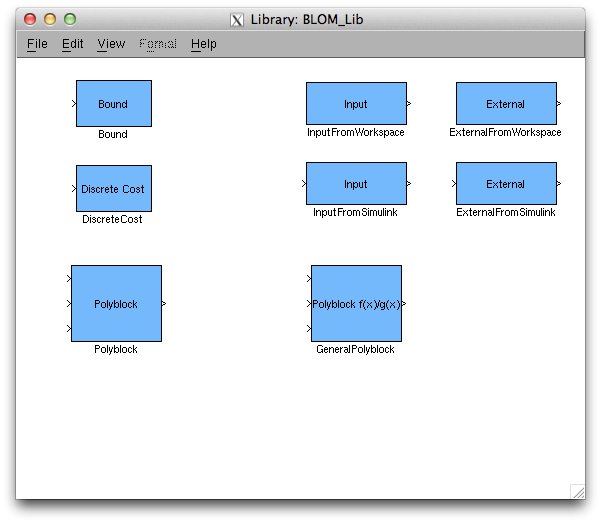
\includegraphics[width=100mm]{figures/BLOM_Lib.png}
\vspace{-40pt}
\end{figure}•

\textbu{Externals:} Labels External Variables that can be changed via script or command line for different calls of the solver \\[10pt]
\textbu{Inputs:} Labels Input Variables to be optimized by solver \\[10pt]
\textbu{Bounds:} Sets upper/lower bounds on a variable\\[10pt]
\textbu{Cost:} Cost variable to be minimized.  \\[10pt]
\textbu{Polyblocks:} BLOM's convenient way to create nonlinear functions\\[10pt]

\section{Polyblocks}
BLOM's internal representation of blocks.

$$ y_1=2x^2_1x_2 , \hspace{3mm} y_2=3x_1+x_2^4 $$
\[
P = \begin{bmatrix}
2 & 1 \\
1 & 0 \\
0 & 4
\end{bmatrix}
\hspace{3mm}
K = \begin{bmatrix}
2 & 0 & 0\\
0 & 3 & 1
\end{bmatrix}
\]

$$y_1 = 2x_1+3sin(x_2),  \hspace{3mm} y_2 = 3x_1^2e^{x_3}+0.2tan(x_2)x_4^3$$
\[P= \begin{bmatrix}
1 & 0 & 0 & 0 \\
0 & \text{BLOM\_FunctionCode(`sin')} & 0 & 0\\
2 & 0 & \text{BLOM\_FunctionCode(`exp')} & 0 \\
0 & \text{BLOM\_FunctionCode(`tan')} & 0 & 3
\end{bmatrix}
\]
\section{Setting Up BLOM on Your Computer}
\begin{enumerate}
\item \url{http://mpclab.net/Trac/wiki/SVNsetup} Here are instructions on how to get SVN and how to get BLOM running
\item in command line, \texttt{svn checkout http://www.mpclab.net/BLOM/ \red{desired\_directory}}
\item Each time you open up BLOM, make sure to get the latest version by typing \texttt{svn update} within that folder (or update through TortoiseSVN)
\item On Mac or Linux machines, you may need to compile IPOPT and then run \texttt{BLOM\_Setup} (Instructions for doing so at \url{http://mpclab.net/Trac/wiki/CompilingIpopt})

\end{enumerate}•


\clearpage
\section{Creating Model Example}
\vspace{-20pt}$$\max  f(x)=3x_1+x_2-x_3^2+2x_3$$
$$x_1^2+x_2^2\leq5$$
$$x_1-x_2\leq1$$
$$x_3\geq0$$

\begin{figure}[H]
\textbu{Step 1:} Place Input and External Blocks for input and external variables
\center
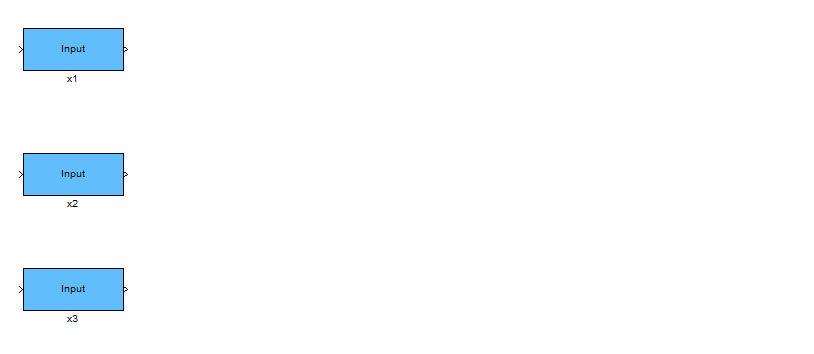
\includegraphics[width=120mm]{figures/Example_Step1.png}
\end{figure}
\begin{figure}[H]
\textbu{Step 2:} For each bound limitation and cost function, drag and drop math blocks to satisfy equations.  Use subsystems and/or polyblocks as needed
\center
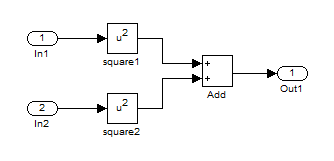
\includegraphics[width=50mm]{figures/Example_Step2_1_subsys.png}
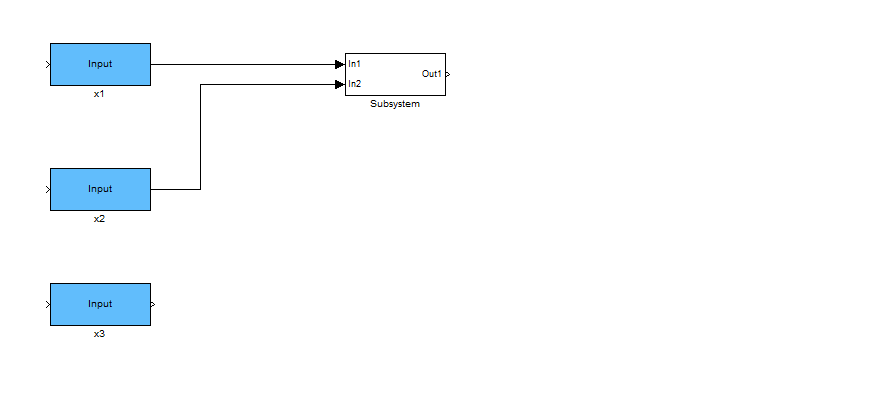
\includegraphics[width=120mm]{figures/Example_Step2_1.png}
\end{figure}
\begin{figure}[H]
\textbu{Step 3:} Attach bound and cost blocks and set limits/time relevances
\center
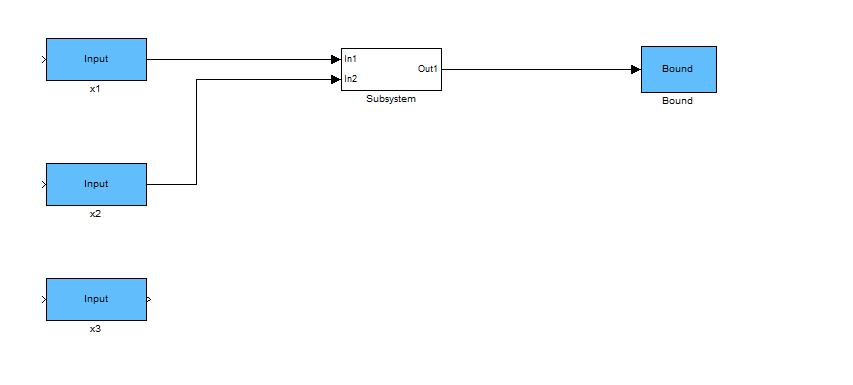
\includegraphics[width=120mm]{figures/Example_Step3_1.png}
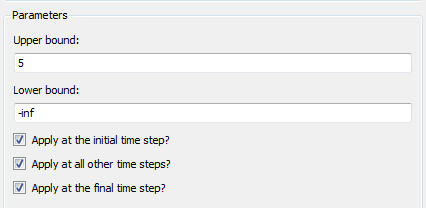
\includegraphics[width=60mm]{figures/Example_Step3_1_bound.png}
\end{figure}
\begin{figure}[H]
Repeat steps 2 and 3 as necessary
\center
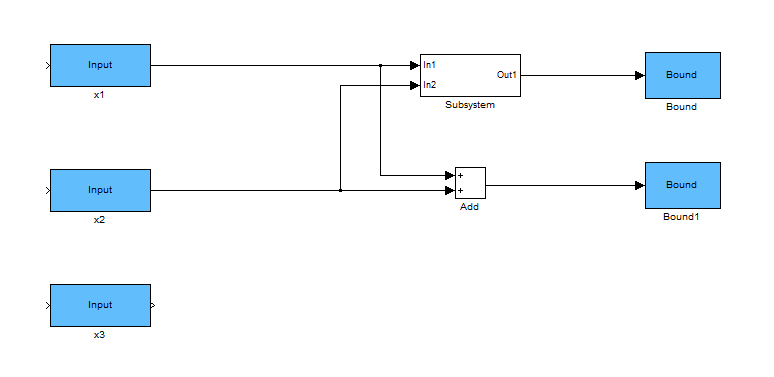
\includegraphics[width=120mm]{figures/Example_Step3_2.png}
\end{figure}
\begin{figure}[H]
\center
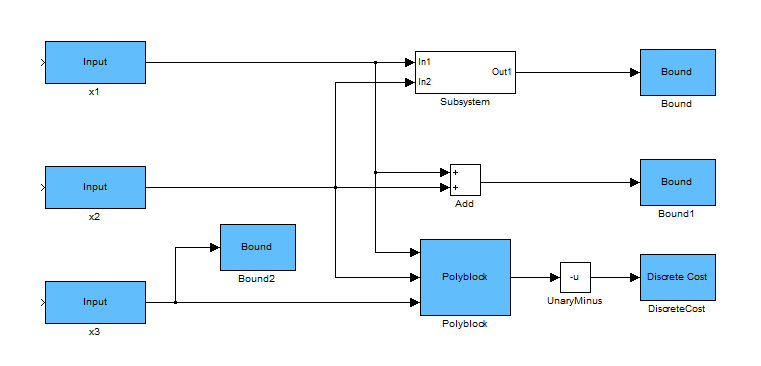
\includegraphics[width=120mm]{figures/Example_final.png}
\end{figure}

\section{Calling BLOM}
\begin{enumerate}
\item Always remember to run \texttt{BLOM\_addpath} to add all the BLOM related files into your path
\item Create model in simulink 
\item \texttt{BLOM\_SetDataLogging(\red{`ModelName'})}
\item \texttt{ModelSpec = BLOM\_ExtractModel(\red{`ModelName'}, \red{\#timesteps})}
\item \texttt{[RunResults ResultsVec] = BLOM\_RunModel(ModelSpec)}
\item \texttt{[OptGuess ExtVars InitialStates ] = BLOM\_SplitResults(ModelSpec,RunResults)}
\item \texttt{SolverStruct = BLOM\_ExportToSolver(ModelSpec,\red{`Solver'})}
\item \texttt{SolverStructData =  BLOM\_SetProblemData(SolverStruct,ModelSpec,OptGuess, ExtVars, InitialStates)}
\item \texttt{SolverResult  =  BLOM\_RunSolver(SolverStructData,ModelSpec)}
\end{enumerate}•
\textbu{Using Externals:} Items 7-9 can be run in a loop using outputs from \texttt{SolverResult} to populate \texttt{OptGuess} and \texttt{InitialStates} in subsequent iterations.  \texttt{OptGuess}, \texttt{ExtVars}, and \texttt{InitialStates} can all be filled in from the command line (e.g. \texttt{ExtVars.x1=5}, and \texttt{OptGuess=SolverResult})



\section{Optimizing Your Model}
\begin{itemize}
\item Use fewer blocks.  Outputs of blocks (with the exception of subsystems, from/goto tags, mux/demux) represent variables.  Having fewer blocks and therefore fewer variables allows for faster computation.
\item Switch to polyblocks.  Converting groups of mathematical operations into polyblocks can also reduce the number of variables
\item For polyblocks with sparse entries, create matrices using Matlab function sparse.  This reduces memory storage and computations are optimized within Matlab.
\end{itemize}•

\clearpage
\section{Currently Supported Simulink Blocks}
\begin{multicols}{2}
\begin{itemize*}	
\item Sum, Add, Subtract 
\item Product, Multiply, Divide
\item Gain
\item Unary Minus
\item Bias
\item Math
\vspace{-5pt}
	\begin{itemize*}
	\item square
	\item sqrt
	\item reciprocal
	\item exp
	\item 10\string^u
	\item log
	\item log10
	\item magnitude\string^2 (Reals only)
	\item 1/sqrt, rsqrt
	\item hypot
	\end{itemize*}•
\item Trigonometry
\vspace{-5pt}
	\begin{itemize*}
	\item sin
	\item cos
	\item tan
	\item asin
	\item acos
	\item atan
	\item sincos
	\end{itemize*}•
\item Polynomial
\item Constant
\item Unit Delay
\item Subsystem
\item From, Goto
\item Mux, Demux
\end{itemize*}•

\end{multicols}

\end{document}